\section{Machine learning}

\subsection{Inleiding}
Een zelflerend systeem is een algoritme gebaseerd op machine learning. Machine learning werd door Arthur Samuel, een pionier op dit gebied, gedefinieerd als: 
\textit{A field of study that gives computers the ability to learn without being explicitly programmed.} \cite{ArthurSamuel} 
In tegenstelling tot de eerder genoemde algoritmes is een zelflerend systeem in staat zichzelf te verbeteren. Hierdoor kan het taken uitvoeren waarbij reguliere algoritmes tekort schieten. We zullen in dit hoofdstuk de volgende vraag beantwoorden: \textit{Wat zijn zelflerende algoritmes en waarin verschillen ze van reguliere algoritmes?}

\begin{figure}[h]
  \centering
    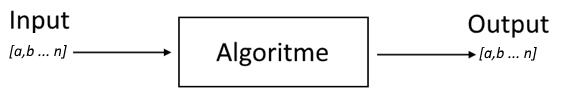
\includegraphics[width=\textwidth]{algorithm1.png}
  \caption{Schematische weergave van een zelflerend systeem}
  \label{fig:algorithm1}
\end{figure}

In figuur \ref{fig:algorithm1}  is een schematische weergave van een zelflerend systeem afgebeeld. Bepaalde input data gaat het systeem in en bepaalde output data komt het systeem uit. De input en output data bestaan uit \'e\'en datatype of uit meerdere datatypen. Als de input simpelweg een reeks getallen betreft, zal dit direct als input gebruikt kunnen worden. In het geval dat de input uit een ander datatype bestaat, zoals een plaatje, zal dit omgezet moeten worden in een reeks getallen voordat het door een zelflerend systeem gebruikt kan worden. Het algoritme zal deze getallen bewerken tot de gewenste output. Deze output wordt eveneens in getallen gegeven. Waar nodig zullen deze getallen dus weer moeten worden omgezet tot het gewenste datatype.

Er zijn veel verschillende algoritmes die gebruikt kunnen worden voor een zelflerend systeem. Elk algoritme heeft voor- en nadelen en is geschikt voor andere doeleinden. Een aantal van deze algoritmes zullen we in het volgende hoofdstuk (hoofdstuk \ref{chapter:MLA}) bespreken.

\subsection{Training}

Een zelflerend systeem begint in de meeste gevallen zonder enige kennis van de data. Om de gewenste output te kunnen produceren is het dus nodig om het systeem eerst input data te geven zodat het kan leren. Dit proces wordt het \textbf{trainen} genoemd. Voor het trainen van een zelflerend systeem is training data nodig. Deze data moet gelijk of gelijkwaardig zijn aan de echte data. De training data kan in veel verschillende vormen voorkomen en de manier van trainen is afhankelijk van de vorm van de (training) data. In figuur \ref{fig:algorithm2}  is te zien dat het trainen los staat van het algoritme. Dit verschil zullen we in het volgende hoofdstuk wat duidelijker maken. 
Er zijn drie prominente manieren waarop een zelflerend systeem kan leren: \textbf{supervised}, \textbf{unsupervised} en \textbf{reinforcement learning}.

\begin{figure}[H]
  \centering
    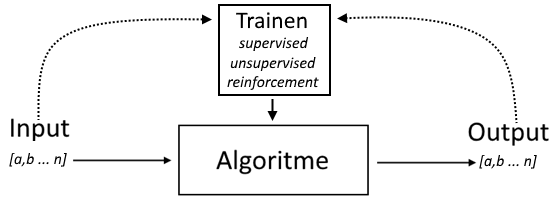
\includegraphics[width=\textwidth]{algorithm2.png}
  \caption{Schematische weergave van een zelflerend systeem}
  \label{fig:algorithm2}
\end{figure}

\subsubsection{Supervised Learning}
In het geval van supervised learning heb je te maken met \textbf{labeled} training data. Anders gezegd: van een bepaalde input is de gewenste output al bekend. Een klassiek voorbeeld van een labeled dataset is een dataset van huisprijzen en huiseigenschappen (zie figuur \ref{fig:LabeledDataset}).

\begin{table}[h]
\centering
\begin{tabular}{llll}
\hline
\multicolumn{1}{c}{\multirow{2}{*}{Huisprijs (output)}} & \multicolumn{3}{c}{Huiseigenschappen (input)} \\
\multicolumn{1}{c}{} & \multicolumn{1}{c}{Woonoppervlakte} & \multicolumn{1}{c}{Perceeloppervlakte} & \multicolumn{1}{c}{Aantal Kamers} \\ \hline
€ 519.000 & 124 m² & 311 m² & 4 \\
€ 569.000 & 133 m² & 309 m² & 5 \\
€ 569.500 & 170 m² & 310 m² & 6 \\ \hline
\end{tabular}
\caption{Labeled dataset Bron: http://www.funda.nl/koop/huizen/ }
\label{fig:LabeledDataset}
\end{table}
Bij de training dataset van tabel \ref{fig:LabeledDataset} is de gegeven input de huiseigenschappen en de gewenste output de huisprijs. Het systeem wordt met deze dataset getraind. Hierdoor leert het een output te produceren die steeds dichter bij de gewenste output ligt. Als er een verband bestaat tussen de huiseigenschappen en de huisprijs, wat waarschijnlijk het geval is, zal het zelflerende systeem na genoeg trainen in staat zijn zelf bij nieuwe huiseigenschappen een huisprijs te voorspellen. \cite{MLCourse1}

\subsubsection{Unsupervised Learning}
Unsupervised learning kan gebruikt worden bij een \textbf{unlabeled} dataset, ofwel een dataset waarbij de data niet geclassificeerd is en er geen gewenste output bekend is. Als je een dataset hebt van heel veel niet-geordende foto's is het niet mogelijk om dit te classificeren. Als een deel van de dataset gelabeld wordt, zal met behulp van supervised learning de rest van de dataset geclassificeerd kunnen worden. Dit is echter in veel gevallen niet mogelijk, bijvoorbeeld doordat de dataset enorm groot is of er zodanig veel verschillende groepen bestaan dat het menselijk niet mogelijk is ook maar een deel te labelen. Ook kan het zo zijn dat men niet weet of er een verband aanwezig is. 
Kortom: unsupervised learning wordt gebruikt voor het classificeren van data, zonder dat er groepen vooraf gedefinieerd zijn. Met behulp van deze vorm van training kunnen in een grote dataset verbanden worden ontdekt, die men misschien niet zonder hulp had kunnen achterhalen.\cite{MLCourse2}

\subsubsection{Reinforcement Learning}
Reinforcement learning is een zeer specifieke soort van leren. Er is bij deze vorm van learning geen dataset met input data, maar is er een bepaalde \textbf{context}. In deze context bevindt zich een \textbf{agent}. Een agent is een object dat bepaalde opdrachten kan uitvoeren. De context is een wereld waarin deze agent zich bevindt. Door de agent bij bepaalde acties pluspunten of minpunten te geven kun je bepaald gedrag bevorderen.  

\begin{figure}[h]
  \centering
    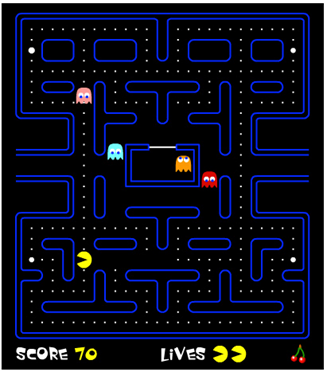
\includegraphics[width=0.5\textwidth]{pacman.png}
  \caption{Pac-Man}
  \label{fig:Pacman}
\end{figure}

In figuur \ref{fig:Pacman} is het spel Pac-Man te zien. Op dit spel zou reinforcement learning toegepast kunnen worden. De agent is hierbij pacman, dit is namelijk een object dat bepaalde opdrachten kan uitvoeren, zoals: beweeg naar links. De context is hierbij het level, ofwel: de positie van de muren (de blauwe obstakels), de posities van de ghosts (de gekleurde vijanden), de posities van de pac-dots (de kleine stipjes) en de posities van de power-pellets (de grotere stipjes). Het eten van de pac-dots is positief, het geraakt worden door de ghosts is negatief. Door reinforcement learing toe te passen op het spel zal de agent steeds beter worden in het spelen van het spel. 

\subsection{Normaliseren van data}
Zoals ook in tabel \ref{fig:LabeledDataset} te zien is, kunnen verschillende inputs erg van elkaar verschillen qua grootte. Zo zal het aantal kamers nooit in de buurt komen van het oppervlak. Uiteindelijk zou dit een probleem kunnen veroorzaken bij de berekeningen van het systeem. Een groot getal zou namelijk een veel groter aandeel kunnen hebben alleen omdat het getal zoveel groter is. Het is daarom gebruikelijk de inputs te normaliseren. Dit houdt in dat de inputs zullen veranderen in een getal met een waarde binnen een bepaald gebied, zodat alle verschillende inputs eerlijk met elkaar vergeleken kunnen worden. Je zou bijvoorbeeld voor de oppervlaktes kunnen stellen dat alle waardes tussen 100 m² en 1000 m² zullen liggen. Aan een input van 500 m² zou je dan een waarde van 5 kunnen geven.

\subsection{Conclusie}
Zelflerende computersystemen zijn algoritmes gebaseerd op machine learning. Een zelflerend systeem verschilt van reguliere algoritmes zoals breadth-first search en depth-first search doordat ze in staat zijn zichzelf te verbeteren.
